\chapter{Multiple Importance Sampling Compensation}
\label{ch:mis_compensation}
This chapter will cover the theory behind MIS compensation as proposed by Karl\'ik et al. in~\cite{Karlik2019}.
First the basic idea of MIS compensation will be explained after which the variance reduction will be proven.

As we can see in figure~\ref{fig:pdf_comparison} when we use our pdfs regularly with the balance heuristic
the resulting pdf is too defensive as the high values are undersampled and the low values are oversampled.
The name for their techniques comes from the compensation for the averaging of the balance heuristic.
One resulting pdf of their approach can be seen in figure~\ref{fig:optimized_mis}.

\begin{figure}[h]
    \centering
    \begin{subfigure}[b]{.3\textwidth}
        \centering
        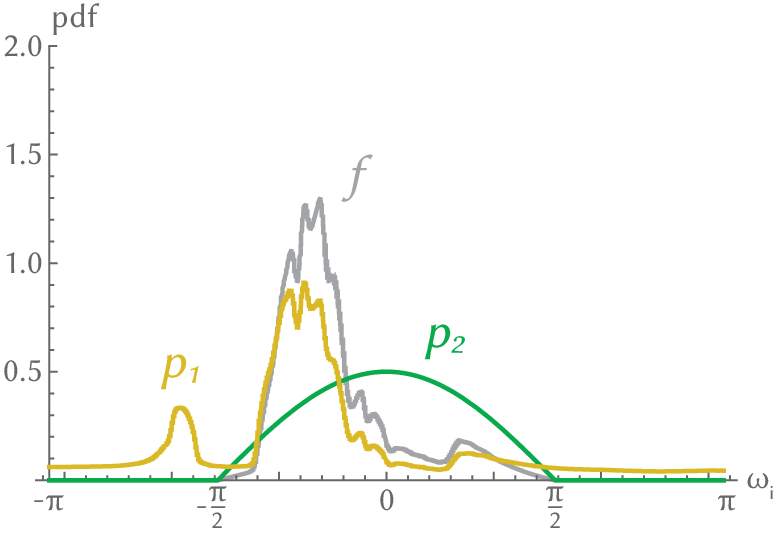
\includegraphics[width=\textwidth]{images/original_setup.png}
        \caption{Original pdfs}
        \label{fig:original_setup}
    \end{subfigure}
    ~
    \begin{subfigure}[b]{.3\textwidth}
        \centering
        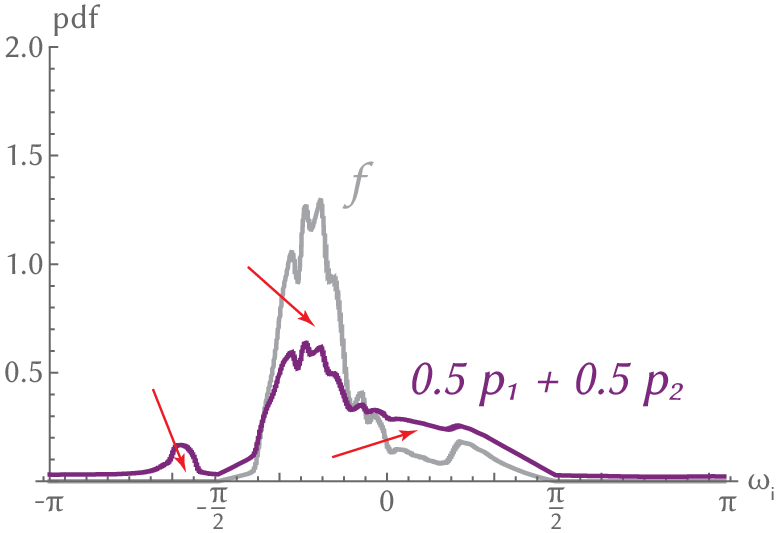
\includegraphics[width=\textwidth]{images/mis_setup.png}
        \caption{Original MIS}
        \label{fig:original_mis}
    \end{subfigure}
    \\
    \begin{subfigure}[b]{.3\textwidth}
        \centering
        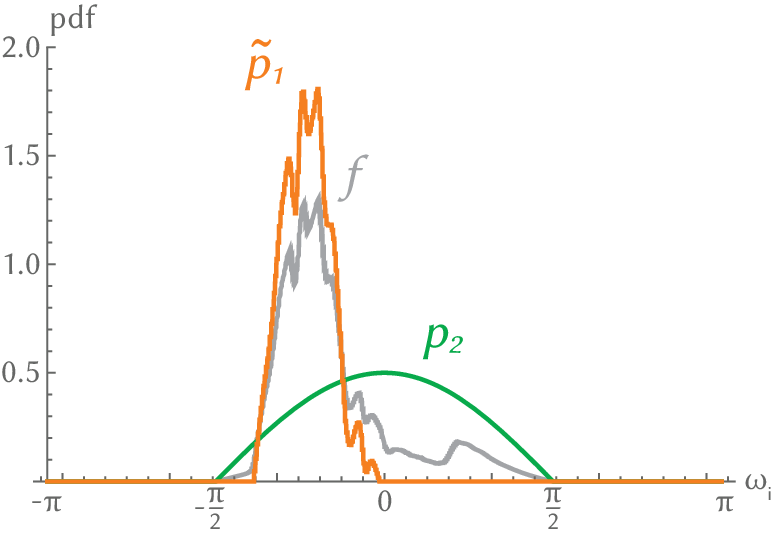
\includegraphics[width=\textwidth]{images/optimized_setup.png}
        \caption{Optimized pdfs
        \label{fig:optimized_setup}}
    \end{subfigure}
    ~
    \begin{subfigure}[b]{.3\textwidth}
        \centering
        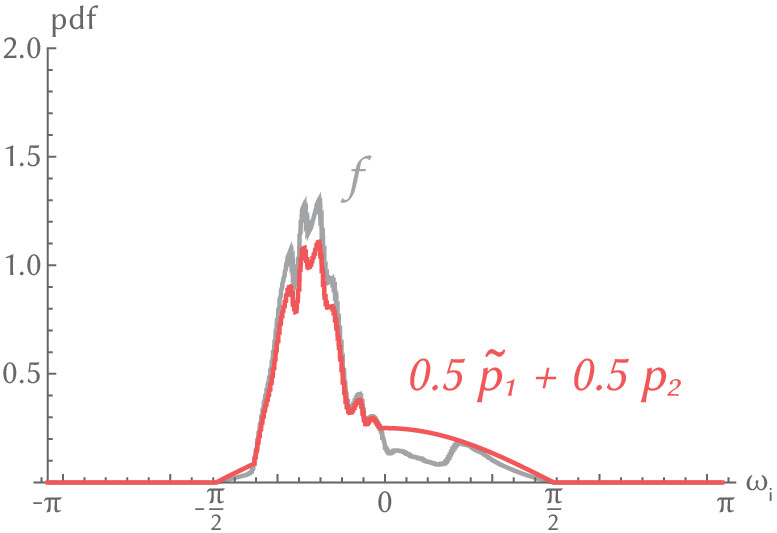
\includegraphics[width=\textwidth]{images/mis_optimized.png}
        \caption{Optimized MIS}
        \label{fig:optimized_mis}
    \end{subfigure}
    \caption{Comparison of the original pdfs without compensation~(\ref{fig:original_setup})
    and how the combined pdf looks like with the balance heuristic~(\ref{fig:original_mis})
    with the modified pdf~(\ref{fig:optimized_setup}) and the balance heuristic using the optimized pdf~(\ref{fig:optimized_mis}).
    f (gray) is the function we want to integrate.
    Figure~\ref{fig:original_mis} shows that the high values are undersampled and the low values are oversampled (see the red arrows).
    The optimized pdfs match the integrand much better when using MIS as seen in figure~\ref{fig:optimized_mis}.
    Figures taken from~\cite[Figure~2]{Karlik2019}.}
    \label{fig:pdf_comparison}
\end{figure}

From a given set of samplers $ T $ they pick one sampler $ t \in T $ and call its pdf $ p_t $ the free pdf that will be used for compensation
so that the combined pdf reduces the variance when used with the balance heuristic.

In an optimal solution the combined pdf $ p_{eff}(x) = f(x)/F $ would lead to zero variance as shown in equation~\ref{eq:zero_variance}.
For the purposes of MIS compensation the combined pdf can also be written as $ p_{eff}(x) = q(x) + c_t p_t(x) $ where $ q(x) = \sum_{i \in T/\{t\}} c_i p_i(x) $
and $ p_t $ is the free pdf with $ c_t $ being its fraction of the total samples.
Whe can reorder to get a formula for
\begin{equation}
    \label{eq:compensated_pdf}
    p_t(x) = \frac{f(x)}{c_t F} - \frac{q(x)}{c_t}.
\end{equation}
This however does not guarantee that $ p_t $ is a valid pdf,
for this they clamped and normalized it and got this formula:
\begin{equation}
    \label{eq:valid_compensated_pdf}
    \tilde{p}_t(x) = \frac{1}{b} max\{0, p_t(x)\}
\end{equation}
with a normalization factor of $ b = \int_X max\{0, p_t(x)\} dx $.

Their compensated pdf fills the gap between the other samplers and the target function $ f(x) $
since it effectively samples only the parts that the other samplers missed in regard to $ f(x) $.
Whenever $ f(x) > 0 $ also $ p_{eff}(x) > 0 $ has to hold true for it to be unbiased.
When we assume $ q(x) = 0 $ then $ p_t(x) > 0 $, because of its definition~\ref{eq:compensated_pdf}.
If $ q(x) > 0 $ then $ p_t(x) $ could become $ 0 $, but then still $ p_{eff}(x) > 0 $ would be the case.
So the combined pdf is valid but it doesn't guarantee to reduce variance, because of the max operator and the re-normalization.


\section{Optimality}
\label{sec:misc_optimality}
In this section we want to find the truly optimal pdf $ p_t^*(x) $ for our free pdf.
First we look at the variance
which can be written as $ E(x^2) - E(x)^2 $ that equals in our case $ J(p) - F^2 $ with $ J(p) = \int_X \frac{f(x)^2}{q(x) + c_t p(x)} $.
The optimal compensating pdf would then be $ p_t^*(x) = \underset{p}{arg~min}~J(p) $.
To make sure $ p_t^*(x) $ is a valid pds we also set these two constraints $$ p_t^*(x) > 0 \text{, and } \int_X p_t^*(x) dx = 1 $$
In the original paper~\cite{Karlik2019} they used the Karush-Kuhn-Tucker constraints
to derive the optimal solution as $$ p_t^{\pm}(x) = \frac{f(x)}{\sqrt{c_t \lambda}} - \frac{q(x)}{c_t},~p_t^*(x) = max\{0, p_t^{\pm}(x)\}. $$
$ \lambda $ is the Lagrange multiplier and ensures normalization.\\
Because of the max operator there is no analytical formulation for the solution and an iterative calculation is impractical in practice,
but if the MIS-compensated solution from equation~\ref{eq:valid_compensated_pdf} is close-enough to the optimal one it can be used instead.
The next section will show that the compensated solution is indeed often similar to the optimal one.


\subsection{Bounds for the MIS-compensated solution}



To show the similarity of the optimal solution and the MIS-compensated one we derive following bounds \dots by \dots (appendix B)
With eq. 9 we can easily see that the optimal and the compensated solution are equal and the lower bound applies. (just input into 9, fulfill conditions)
with this we can assume that the optimal solution is often not far from the compensated one.
In case they are not the same we want to see how badly using the compensated pdf over the optimal one can increase variance
the highest increase would be 1 / ct over the optimal solution.
to get a concrete number for the introduced variance multiple scenes were tested with the worst result being 1.6 times

They showed that the compensated pdf is often similar to the optimal one.
In case they are not the same it is expensive to calculate the optimal pdf since it involves iteratively evaluating the integral and checking if the conditions hold true
the mis-compensated solution can be used because it is easy to calculate with an approximation of F and is still a good overall solution.

\todo{is it okay to refer to the original paper for the derivation of the optimal solution (appendix proovs). Yes it is, the idea should be clear here and the reference also to the paper.}

\todo{show how F will be approximated by $\lambda$. maybe no approach to approximation is shown}

\todo{Explain their work. Formulas should be clearly explained.}